\chapter{Experimental Setup} \label{Chapter4}

\section{RAC components} \label{RAC components}
In order to provide a solution to the goals stated in Section \ref{Business context} it is important to obtain a good understanding of all aspects that play a role within the RAC. A short description of all hardware and software aspects is given below. It is possible that not all described components are relevant to this project. Nevertheless, some terms may be used throughout this thesis and therefore a brief description of these components can be helpful. Section \ref{Hardware} gives an overview of the hardware components within the RAC, the robotic arm, vision camera and AnyFeeder. The robotic arm will be discussed more thoroughly because that aspect requires the most maintenance and is therefore more interesting. Section \ref{Software} gives an overview of all software components within the RAC, V+\textsuperscript{\tiny{TM}}, ACE\textsuperscript{\tiny{TM}}, and AdeptSight\textsuperscript{\tiny{TM}} that play a role by designing the CBM tool.

\subsection{Hardware} \label{Hardware}
As mentioned before, the RAC consist of several components (AnyFeeder, vision camera, robotic arm, conveyor belt). The vision cameras and the robotic arms are products of Bremer Werk für Montagesysteme (BWM), a company that produces assembly systems, automation systems, and special-purpose machine manufacturing\footnote{https://www.bwm-gmbh.de/en/unternehmen/}. BWM has established the ALs at Philips by installing the RACs and providing controllers to the components. For example, the trajectory that a robotic arm has to execute in order to assemble certain parts of a shave is programmed by BWM. 

The vision guidance system and Adept AnyFeeder\textsuperscript{\tiny{TM}} that are part of RB34 are not discussed in detail. Obtaining data from the AnyFeeder is a complex task that should be performed by Adept programmers and will be outside the scope of this project. Maintenance on the vision guidance system is rare and therefore it is not relevant to predict it.  

The robot arms within RAC RB34 that are used to assemble the shaver units are Adept Cobra s600's with four axis. This is a high-performance Selective Compliance Assembly Robot Arm (SCARA) robot system for mechanical assembly, material handling, packaging, machine tending, screw driving, and other applications that require fast and precise automation. This robot include the Adept SmartController CX\textsuperscript{\tiny{TM}} motion controller, an ultra-compact, high-performance, distributed robot motion controller capable of controlling an entire production line managing multiple robots. Before this project,the Smart Controller was not able to subtract the data from the robot arms. During the project, a programmer from Omron Adept visited Philips and installed a data storing function on the controller especially for this project. In Figure \ref{fig:Cobra s600} and \ref{fig:SmartController} the robot arm and the motion controller are depicted, respectively, and a full description of the hardware is available on the website of Adept\footnote{http://www.adept.com/products/robots}. The most important component within the Omron Adept robot arms that is of importance for this project is described below.
\begin{figure}[ht]
\centering
\begin{subfigure}[b]{0.49\textwidth}
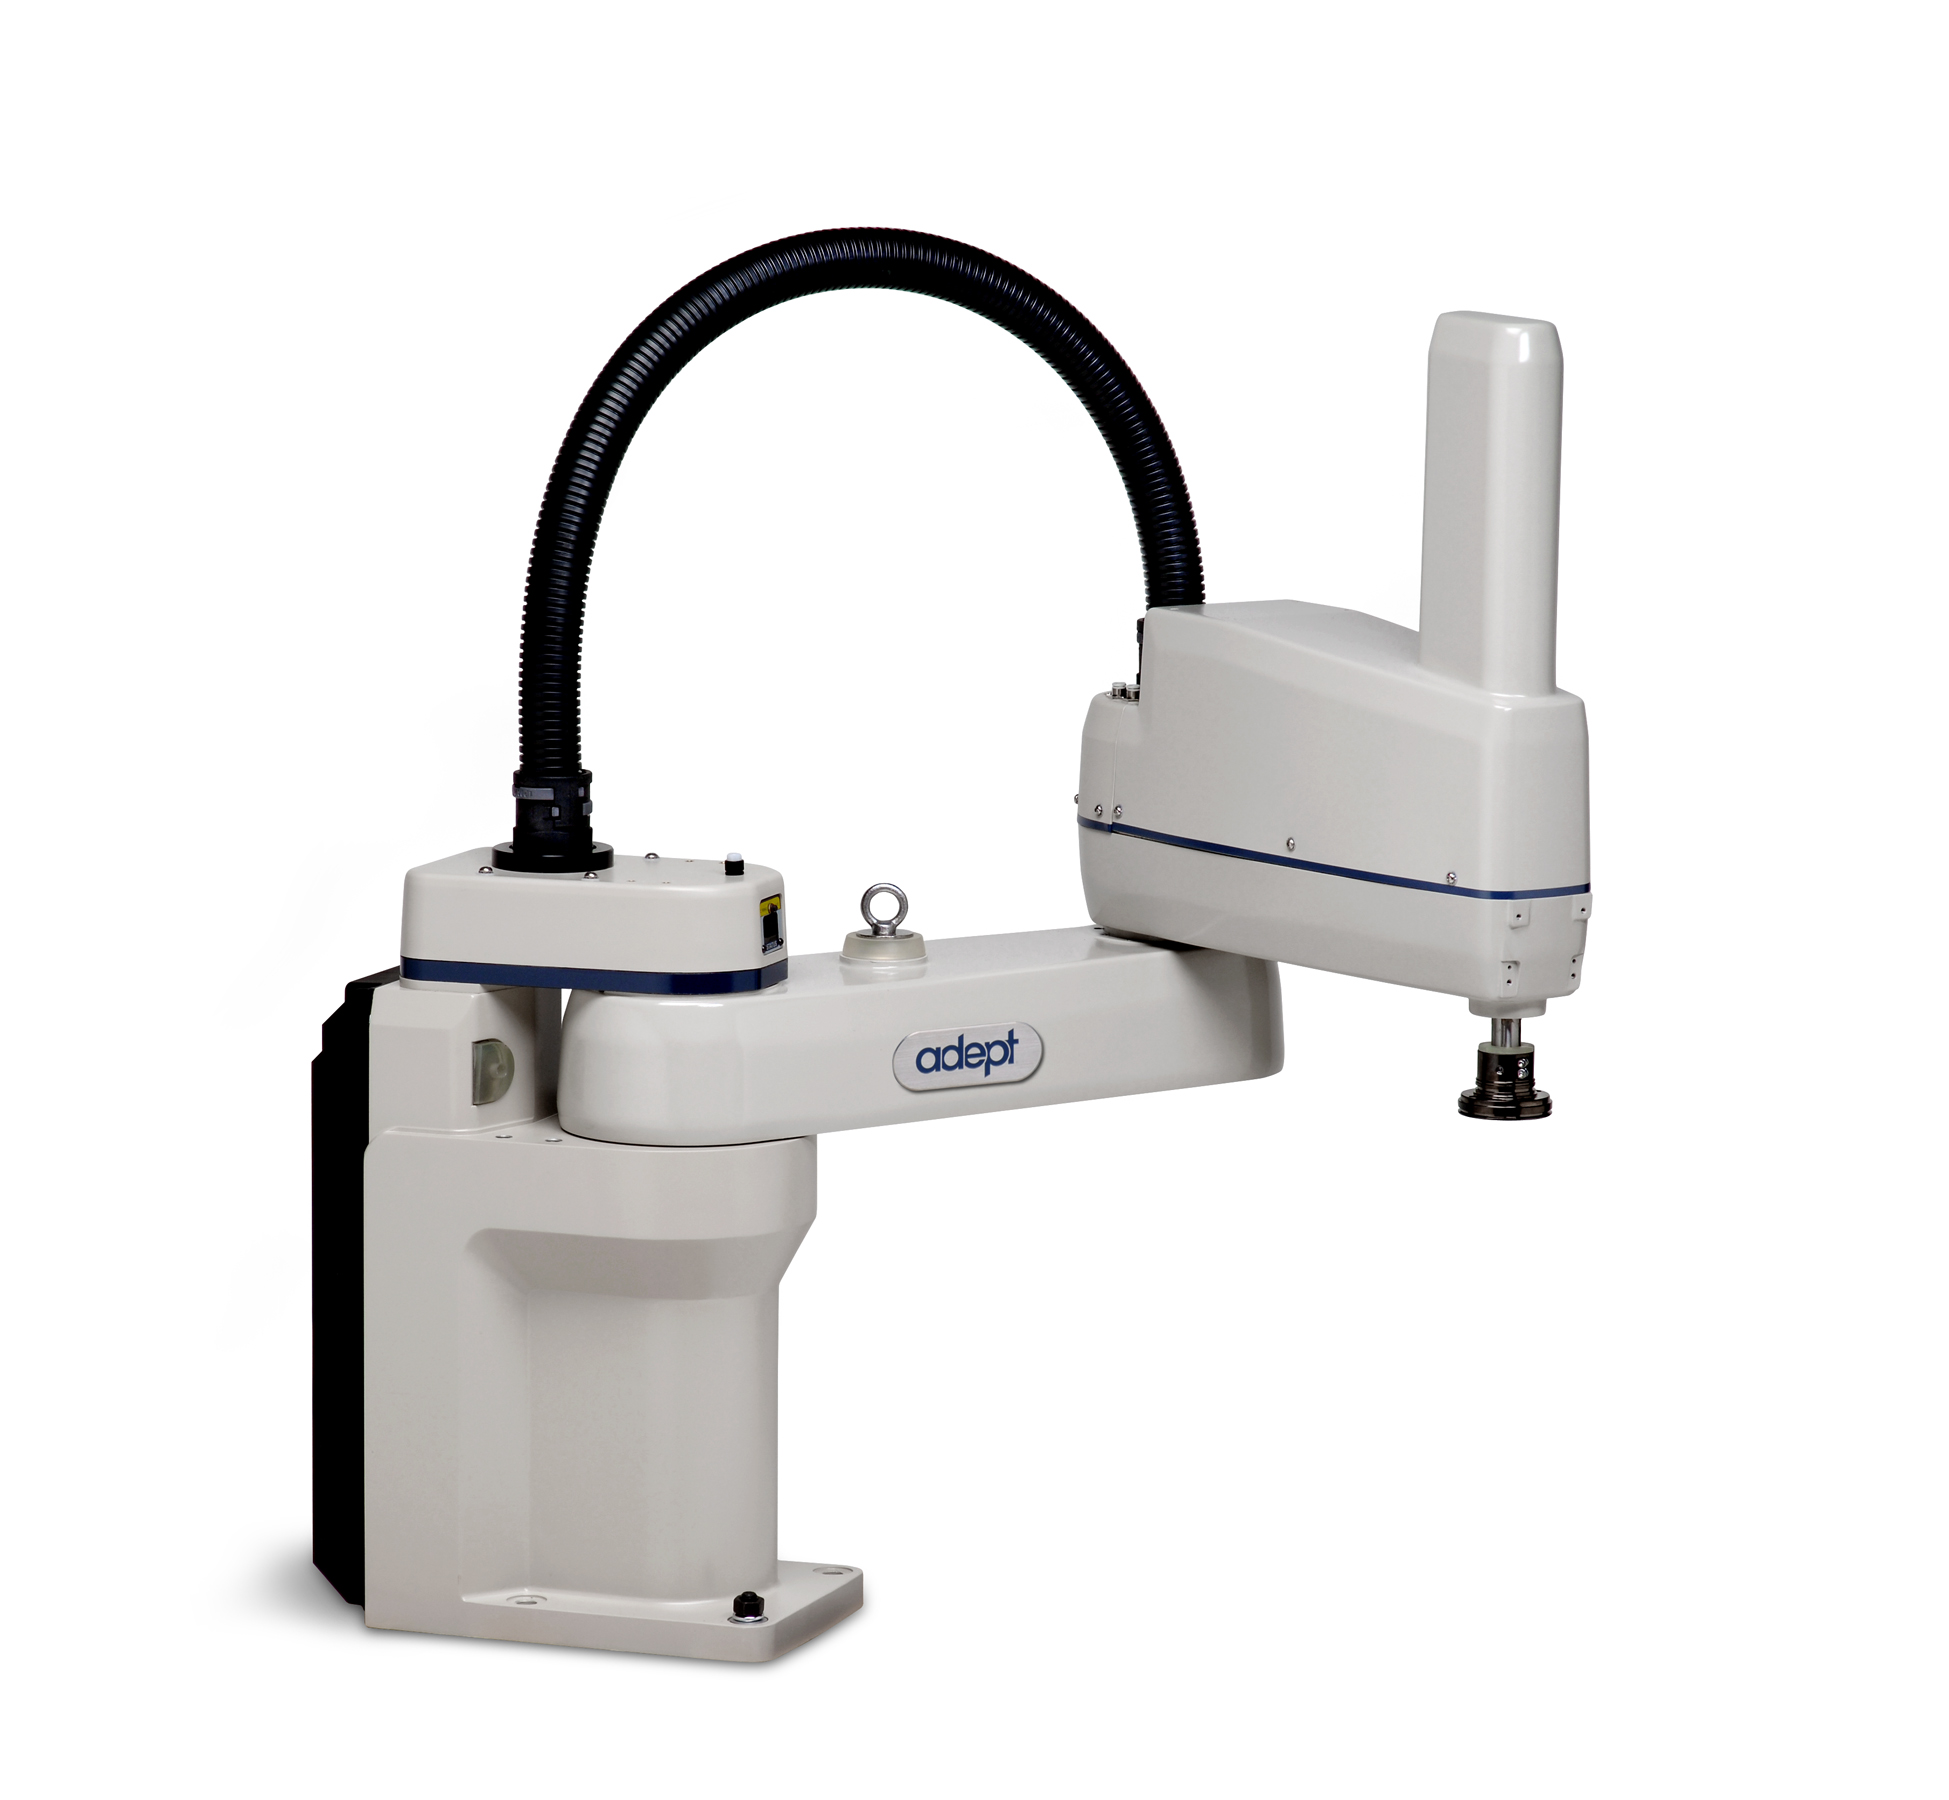
\includegraphics[width=\textwidth]{Figures/Cobra-600}
\caption{Adept Cobra s600}
\label{fig:Cobra s600}
\end{subfigure}
\begin{subfigure}[b]{0.49\textwidth}
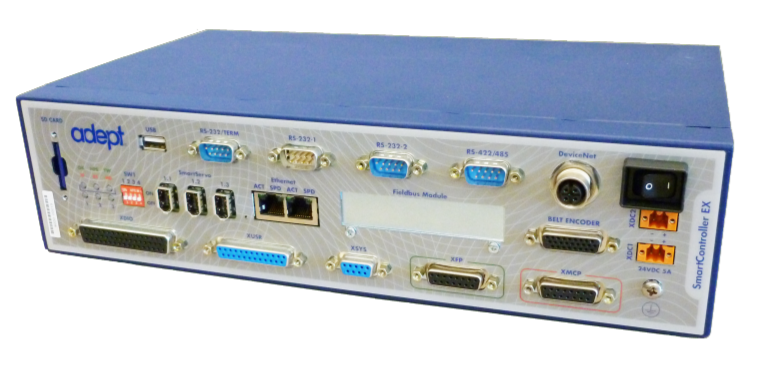
\includegraphics[width=\textwidth]{Figures/SmartController}
\caption{Adept SmartController CX}
\label{fig:SmartController}
\end{subfigure}
\caption[Relevant hardware components of RB34]{Hardware components of RB34}
\label{fig:HardwareComponents}
\end{figure}

\subsubsection{Harmonic drive} \label{Harmonic drive}
Harmonic drive is the brand name of strain wave gears and is a high accuracy gearing component that is the core of the control mechanism of a robot joint. The drive advantages include high gear ratios, high torque capability and good repeatability when repositioning inertial loads. A detailed explanation of harmonic drives can be found online at, for example, the website of Harmonic Drive AG\textsuperscript{\textregistered}\footnote{https://harmonicdrive.de/de/startseite/}.

A harmonic drive has several types of failure modes, and according to \citet{Schafer2005} fatigue fracture of the flex spline is the most common failure mode. \citet{Hauschild2007} describes the friction behavior of harmonic drive actuators with friction compensation methods that reduce the level of apparent friction. One of the consequences of a harmonic drive failure is that lubricates can leak into the motor which is located beneath the harmonic drive. Therefore, if a harmonic drive or its seals fail, the motor will be replaced as well. 

\subsection{Software} \label{Software}
The programming language that is used is V+, a language to provide an integrated solution to all of the programming needs in a robotic workcell, including safety, robot motion, vision operations, force sensing and I/O. It is used to combine the vision guidance software with the control software that is installed on the PC of the RAC. 

AdeptSight\textsuperscript{\tiny{TM}} is an easy-to-use, standalone vision guidance and inspection package and comes complete with all the necessary accessories. The software includes a powerful framework that can be used to develop customized vision guidance and inspection applications. 

The interaction with operators at the RACs is provided by an interface called ACE (Automation Control Environment) which features an integrated environment for robot and control. Data is available for every robotic arm motor regarding temperature, torque, voltage, position error and duty cycle and can be displayed on the Human Machine Interface (HMI) which is connected with the control system of a RAC. The different types of data and their relevance are discussed in Section \ref{Data Gathering}.

\section{Data gathering} \label{Data Gathering}
Data that is useful for the execution of the research will be presented. By analyzing the available data, the relevant data to investigate can be determined and research question one will be answered. There are two ways of obtaining robot and motor data from the RAC described in the ACE User's Guide, 3.7.x \footnote{http://www1.adept.com/main/ke/data/pdf\_web/ace\_ug.pdf}. Firstly, the System Monitor tool is used to perform real-time monitoring of objects in the workspace. Secondly, the Data Collection tool is used to collect values on the servo node at up to the servo rate of 8 KHz. Data types available from the tools overlap each other. A complete list of all data types that are available, according to the Adept ACE User's Guide, can be found in Appendix \ref{AppendixB}. From those types of data it should be determined which type is relevant and is able to predict  maintenance. Since all Cobra s600  robots within the AL are identical and execute similar tasks, it is assumed that the same data type(s) will predict similar maintenance for all Cobra s600 robots.

Only the newer assembly lines within Philips are equipped with the Adept ACE software. The older lines, which require more maintenance, have an older software program installed, called Adept Desktop. This software program is not able to log or collect any data that is available from the robot arms. Therefore, an engineer from Omron Adept developed a V+ program that can be loaded on every RAC controller and is able to collect specific parameters one time per second. Data that can be collected by this program is listed in Table \ref{tab:CollectableData}. A description of what the data entails can be found in Appendix \ref{AppendixB}. To collect data using this program it should be installed on the corresponding RAC controller. Data will be saved on the controllers desktop and can be extracted by connecting a laptop to the controller. This entails that collecting data from a RAC have to be done manually.

\begin{table}[ht]
\begin{center}
\caption[Collectable data types from designed V+ program]{Collectable data types from designed V+ program} \label{tab:CollectableData}
\begin{tabular}[width=\textwidth]{p{0.305\textwidth}|p{0.305\textwidth}|p{0.305\textwidth}}
\multicolumn{3}{c}{Collectable data types} \\
\hline
DC Input & Amplifier Temperature & Harmonic Drive Usage \\
AC Input & Encoder Temperature & Actual Torque \\
Bus Voltage & Duty Cycle & Peak Torque \\
Base Board Temperature & Harmonic Drive Life &Peak Position Error \\
\end{tabular}
\end{center}
\end{table}

One robot arm within RB34 has some undesirable noises during operation and the other robot is working properly. The noisy robot is already on the nomination to be replaced by a new one. However, since the data from this noisy robot is useful for this project, the replacement is postponed until collecting data is no longer necessary. Besides data from RB34, other RACs are investigated as well. Data available from normal operating robot arms are useful in determining normal operating condition. RACs and corresponding robot arms that are investigated during this project are listed in Table \ref{tab:InvestigatedRACs}.

\begin{table}[ht]
\begin{center}
\caption[Investigated RACs with corresponding robot arm types]{Investigated RACs with corresponding robot arm types} \label{tab:InvestigatedRACs}
\begin{tabular}[width=\textwidth]{c|c|c|c}
RAC & Ass. Line & Robot Nr. & Robot type \\ 
\hline
\multirow{2}{*}{RB34} & \multirow{2}{*}{SUA3} & 1 & Cobra s600 \\
& & 2 & Cobra s600 \\
\hline
\multirow{2}{*}{RB33} & \multirow{2}{*}{SUA3} & 1 & Cobra s600 \\
& & 2 & Cobra s600 \\
\hline
\multirow{3}{*}{RB52} & \multirow{3}{*}{SUA4} & 1 & Cobra s600 \\
& & 2 & Cobra s800 \\
& & 3 & Viper 350 \\
\hline
\multirow{2}{*}{RB53} & \multirow{2}{*}{SUA4} & 1 & Cobra s600 \\
& & 2 & Cobra s800 \\
\hline
\multirow{2}{*}{RB72} & \multirow{2}{*}{APV4} & 1 & Cobra s600 \\
& & 2 & Cobra s800 \\
\hline
\multirow{2}{*}{RB73} &\multirow{2}{*}{APV4} & 1 & Cobra s600 \\
& & 2 & Cobra s600 \\
\end{tabular}
\end{center}
\end{table}

